\documentclass[12pt]{article}
\usepackage{amsmath, amssymb, geometry, fancyhdr, tikz}
\geometry{margin=1in}
\pagestyle{fancy}
\fancyhead[L]{\textbf{Discrete Structures}}
\fancyhead[C]{Chapter 4.6 --- RSA vs. Ed25519}
\fancyhead[R]{\textbf{ch\_04\_section\_06\_RSA\_3.tex}}
\usetikzlibrary{positioning}
\usepackage{tikz}
\usetikzlibrary{positioning}

\begin{document}

\begin{center}
    {\LARGE \textbf{From RSA to Ed25519: The Evolution of Digital Locks}}\\[1em]
    {\large Understanding Modern Public-Key Cryptography through Pictures and Intuition}
\end{center}

---

\section*{1. The Big Picture: Why RSA Was Revolutionary}

RSA (1977) was the first practical public-key cryptosystem.
It allowed two people to communicate securely *without ever meeting to share a secret key.*

\vspace{0.5em}
\noindent\textbf{Core idea:}
\[
\text{Encryption: } C = M^e \bmod n,
\qquad
\text{Decryption: } M = C^d \bmod n.
\]
where \(n = p \times q\) for two large primes.

It’s elegant and reliable — but it has one big weakness:  
\textbf{to stay secure, the numbers must be huge.}  
A modern RSA key is often 2048 or 4096 bits long!

---

\section*{2. The New Generation: Elliptic-Curve Cryptography (ECC)}

Elliptic-curve systems (like Ed25519, Curve25519, or ECDSA) keep the same basic \emph{public/private key idea},  
but they use geometry instead of multiplication and factoring.

\[
\text{Public key} = \text{Private key} \times \text{Base point on the curve}.
\]

You can think of it like walking along a strange mathematical landscape — the \emph{elliptic curve}.  
Going forward along the path (multiplying by the private key) is easy,  
but figuring out how far you walked just by looking at the final spot is almost impossible.  
That’s the “elliptic curve discrete logarithm problem.”

---

\section*{3. RSA vs. ECC: A Side-by-Side View}

\begin{center}
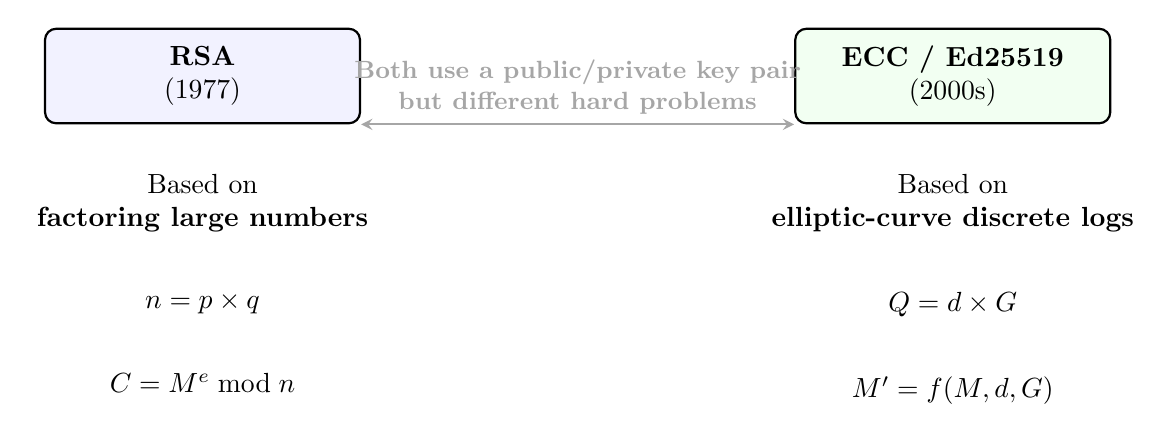
\begin{tikzpicture}[>=stealth, thick, node distance=4.5cm, every node/.style={align=center}]
    % RSA
    \node (rsa) [draw, rounded corners, fill=blue!5, minimum width=4cm, minimum height=1.2cm] {\textbf{RSA} \\ (1977)};
    \node (rsa_math) [below=0.5cm of rsa] {Based on \\ \textbf{factoring large numbers}};
    \node (rsa_key) [below=0.5cm of rsa_math] {\(n = p \times q\)};
    \node (rsa_ops) [below=0.5cm of rsa_key] {\(C = M^e \bmod n\)};
    
    % ECC
    \node (ecc) [draw, rounded corners, fill=green!5, right=5.5cm of rsa, minimum width=4cm, minimum height=1.2cm] {\textbf{ECC / Ed25519} \\ (2000s)};
    \node (ecc_math) [below=0.5cm of ecc] {Based on \\ \textbf{elliptic-curve discrete logs}};
    \node (ecc_key) [below=0.5cm of ecc_math] {\(Q = d \times G\)};
    \node (ecc_ops) [below=0.5cm of ecc_key] {\(M' = f(M, d, G)\)};
    
    % Arrows and caption
    \draw[<->, thick, gray!70] (rsa.south east) -- node[above, midway, sloped, font=\small\bfseries]{Both use a public/private key pair \\ but different hard problems} (ecc.south west);
\end{tikzpicture}
\end{center}

\bigskip

| Concept | RSA | ECC / Ed25519 |
|----------|-----|---------------|
| **Math base** | Multiplying primes, factoring | Geometry on a curve |
| **Hard problem** | Integer factorization | Elliptic curve discrete log |
| **Security growth** | Bigger keys → more security | Same security with much smaller keys |
| **Key size** | 2048 bits typical | 256 bits typical |
| **Speed** | Slower (big exponentiation) | Faster (smaller arithmetic) |
| **Introduced** | 1977 | ~2005 (modern Ed25519 in 2011) |

---

\section*{4. A Visual Metaphor}

\begin{center}
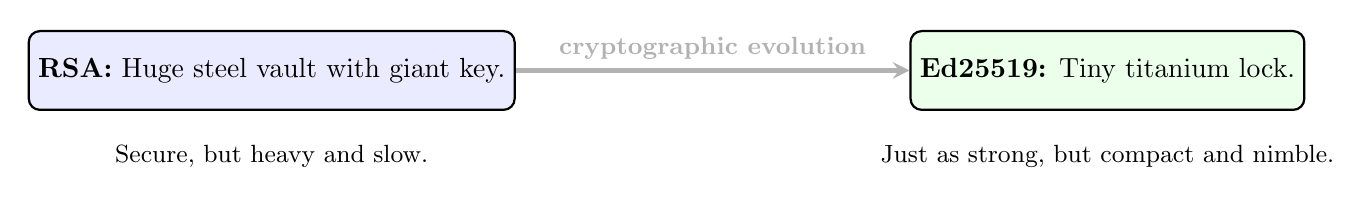
\begin{tikzpicture}[>=stealth, thick, node distance=2cm, every node/.style={align=center}]
    % RSA metaphor
    \node (rsa) [draw, rounded corners, fill=blue!8, minimum width=5cm, minimum height=1cm] {\textbf{RSA:} Huge steel vault with giant key.};
    \node (rsa_note) [below=0.3cm of rsa] {\small Secure, but heavy and slow.};

    % ECC metaphor
    \node (ecc) [draw, rounded corners, fill=green!8, right=5cm of rsa, minimum width=5cm, minimum height=1cm] {\textbf{Ed25519:} Tiny titanium lock.};
    \node (ecc_note) [below=0.3cm of ecc] {\small Just as strong, but compact and nimble.};

    \draw[->, ultra thick, gray!60] (rsa.east) -- node[above, font=\small\bfseries]{cryptographic evolution} (ecc.west);
\end{tikzpicture}
\end{center}

---

\section*{5. What Ed25519 Specifically Does}

Ed25519 is a special case of \emph{Edwards-curve Digital Signature Algorithm (EdDSA)}  
built on the curve called \texttt{Curve25519}.

\begin{itemize}
    \item It’s used for signing and verifying messages, not encrypting them directly.
    \item It’s incredibly fast, especially on modern CPUs.
    \item It avoids many implementation pitfalls of older algorithms.
    \item It provides about the same security as a 3072-bit RSA key — with only 256 bits!
\end{itemize}

\[
\begin{array}{c}
\text{Private key: } k \\
\text{Public key: } A = k \times G \\
\text{Signature: } (R, S) = (r \times G, \; r + H(R, A, M) \times k)
\end{array}
\]
All operations happen on points on the elliptic curve — not with giant integer exponents.

---

\section*{6. Why It Matters}

\begin{itemize}
    \item Smaller keys mean faster connections (think HTTPS, SSH, VPNs).
    \item Signatures are smaller — great for constrained devices or blockchains.
    \item The math is newer, but the logic is the same: one key to lock, one to unlock.
    \item Quantum computers may one day threaten RSA; ECC lasts longer (though not forever).
\end{itemize}

---

\section*{7. Final Comparison Diagram}

\begin{center}
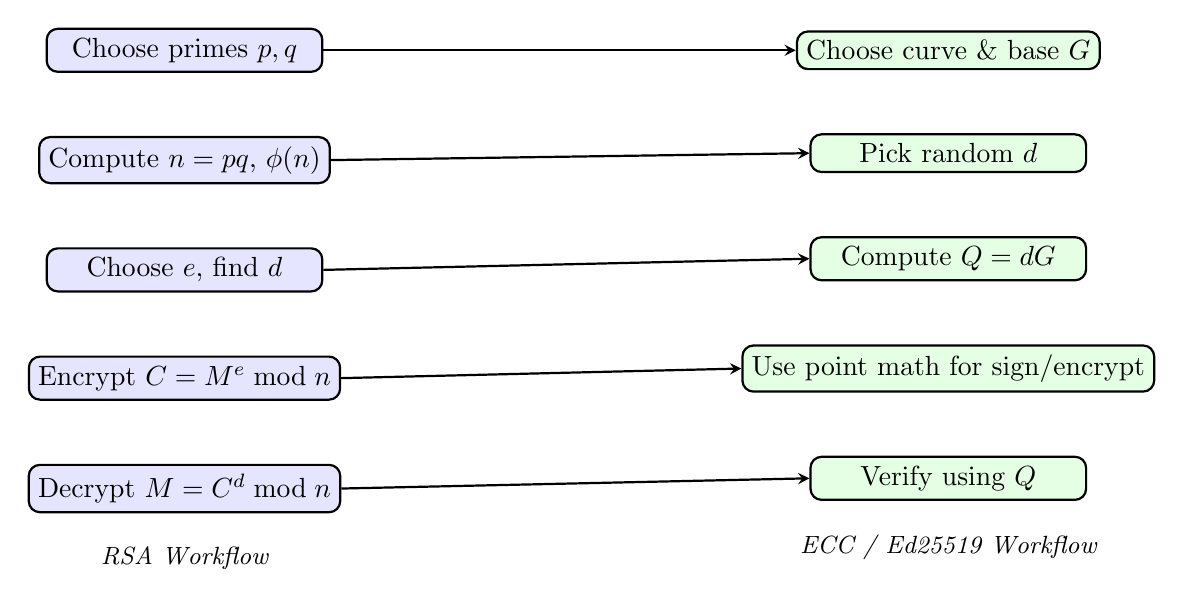
\begin{tikzpicture}[>=stealth, thick, node distance=2cm, every node/.style={align=center, minimum width=3.5cm, rounded corners}]
    % RSA Path
    \node (rsa1) [draw, fill=blue!10] {Choose primes $p,q$};
    \node (rsa2) [below=0.8cm of rsa1, draw, fill=blue!10] {Compute $n=pq$, $\phi(n)$};
    \node (rsa3) [below=0.8cm of rsa2, draw, fill=blue!10] {Choose $e$, find $d$};
    \node (rsa4) [below=0.8cm of rsa3, draw, fill=blue!10] {Encrypt $C=M^e\bmod n$};
    \node (rsa5) [below=0.8cm of rsa4, draw, fill=blue!10] {Decrypt $M=C^d\bmod n$};
    \node (rsa_label) [below=0.3cm of rsa5, font=\small\itshape] {RSA Workflow};

    % ECC Path
    \node (ecc1) [right=6cm of rsa1, draw, fill=green!10] {Choose curve \& base $G$};
    \node (ecc2) [below=0.8cm of ecc1, draw, fill=green!10] {Pick random $d$};
    \node (ecc3) [below=0.8cm of ecc2, draw, fill=green!10] {Compute $Q=dG$};
    \node (ecc4) [below=0.8cm of ecc3, draw, fill=green!10] {Use point math for sign/encrypt};
    \node (ecc5) [below=0.8cm of ecc4, draw, fill=green!10] {Verify using $Q$};
    \node (ecc_label) [below=0.3cm of ecc5, font=\small\itshape] {ECC / Ed25519 Workflow};

    % Connection arrows
    \draw[->, thick] (rsa1.east) -- (ecc1.west);
    \draw[->, thick] (rsa2.east) -- (ecc2.west);
    \draw[->, thick] (rsa3.east) -- (ecc3.west);
    \draw[->, thick] (rsa4.east) -- (ecc4.west);
    \draw[->, thick] (rsa5.east) -- (ecc5.west);
\end{tikzpicture}
\end{center}

---

\section*{8. Epilogue}

RSA is still everywhere — old, wise, and reliable.  
But Ed25519 is like its younger, athletic cousin:
it does the same job, just faster and lighter.

The world keeps both around, because understanding RSA teaches us the bones of cryptography,  
and understanding Ed25519 shows us where the field is going next.

\begin{center}
    \vspace{0.5em}
    \rule{0.7\textwidth}{0.5pt}\\[0.5em]
    \textit{“RSA built the foundation. Elliptic curves built the house.”}
\end{center}

\end{document}

